% This file was created by matlab2tikz.
%
%The latest updates can be retrieved from
%  http://www.mathworks.com/matlabcentral/fileexchange/22022-matlab2tikz-matlab2tikz
%where you can also make suggestions and rate matlab2tikz.
%
\definecolor{mycolor1}{rgb}{1.00000,1.00000,0.00000}%
%
\begin{tikzpicture}

\begin{axis}[%
	width=0.35\linewidth,
	height=0.25\textheight,
	font=\footnotesize,
	scale only axis,
	xmin=3,
	xmax=12,
	xlabel style={font=\color{white!15!black}},
	xlabel={$\tau$},
	ymode=log,
	ymin=1e-05,
	ymax=10,
	yminorticks=true,
	ylabel style={font=\color{white!15!black}, anchor=south west, at={(0.2,0.55)}},
	ylabel={$F$},
	axis background/.style={fill=white},
	title style={font=\bfseries},
	xmajorgrids,
	ymajorgrids,
	yminorgrids,
	legend style={at={(1,1)}, anchor=north east, legend cell align=left, align=left, draw=white!15!black, font=\scriptsize}
]
\addplot [color=blue, line width=1.0pt, mark size=2.0pt, mark=+, mark options={solid, blue}]
  table[row sep=crcr]{%
3	0.85498\\
4	0.48052\\
5	0.26636\\
6	0.1546\\
7	0.08462\\
8	0.04547\\
9	0.02541\\
10	0.01325\\
11	0.00682\\
12	0.00384\\
13	0.00202\\
14	0.00103\\
15	0.00058\\
16	0.00033\\
17	0.00022\\
18	0.00014\\
19	0.0001\\
20	6e-05\\
};
\addlegendentry{RR}

\addplot [color=green, line width=1.0pt, mark size=2.0pt, mark=o, mark options={solid, green}]
  table[row sep=crcr]{%
3	0.84086\\
4	0.16367\\
5	0.02339\\
6	0.00313\\
7	0.00039\\
8	3e-05\\%0\\
9	0\\
10	0\\
11	0\\
12	0\\
13	0\\
14	0\\
15	0\\
16	0\\
17	0\\
18	0\\
19	0\\
20	0\\
};
\addlegendentry{PQ}

\addplot [color=red, line width=1.0pt, mark size=2.0pt, mark=+, mark options={solid, red}]
  table[row sep=crcr]{%
3	0.80513\\
4	0.15542\\
5	0.0195\\%0.01095\\
6	0.0024\\
7	0.00027\\
8	2e-05\\
9	2e-6\\%2e-05\\
10	0\\
11	0\\
12	0\\
13	0\\
14	0\\
15	0\\
16	0\\
17	0\\
18	0\\
19	0\\
20	0\\
};
\addlegendentry{OL}

\addplot [color=black, line width=1.0pt, mark size=2.0pt, mark=x, mark options={solid, black}]
  table[row sep=crcr]{%
3	0.57865\\
4	0.10797\\
5	0.00866\\
6	0.00076\\
7	8e-05\\
8	9e-6\\%0\\
9	0\\
10	0\\
11	0\\
12	0\\
13	0\\
14	0\\
15	0\\
16	0\\
17	0\\
18	0\\
19	0\\
20	0\\
};
\addlegendentry{VI}


\end{axis}
\end{tikzpicture}%